\chapter{Model Inspection, Executable Verification, and Evaluator Reliability}\label{ch:C25}
An executable evaluator can be wrong about what it certifies. TestJack's October 2026 witness construction targets candidates that pass existing tests while violating prompt-grounded requirements~\cite{yao2026testjack}. The resulting conflict is between an operational gate and a task property; it is not resolved by declaring either a test or a language-model reviewer an oracle. This current case motivates the chapter's separation of internal interventions, executable verification, evaluator classification error, and release evidence.

Inspection asks what a model or execution system is doing. Verification asks whether a specified property holds under declared assumptions. The two can support one another, but neither subsumes the other. An interpretable activation pattern does not prove that a tool action is authorized. A passing test does not reveal the complete internal mechanism that produced the artifact. A reliable technical account must identify the property, observation boundary, intervention, and residual uncertainty for each claim.

This chapter connects internal model interventions to executable task validators and evidence-based quality gates. It emphasizes false acceptance, evaluator dependence, and specification gaps because these are the points where apparent assurance can exceed actual support. Every proposed test remains a proposed experiment unless execution evidence is available.

\section{Properties observations and assurance boundaries}\label{sec:C25:properties}
Start with a property $P(x,e)$ of artifact or action $x$ in environment $e$. A verifier $V$ observes a projection $o(x,e)$ and returns accept, reject, or unresolved. The projection can omit decisive state. For example, a screenshot may not show a file's location, and a test log may not identify the artifact revision. No verifier can reliably recover distinctions absent from its observation without additional assumptions or queries.

This leads to three separate questions. Is the property well defined? Does the observation contain evidence sufficient to judge it? Does the verifier use that evidence correctly? A weak result at the third stage can be improved by a stronger judge. A failure at the second stage requires a better observation interface. A failure at the first stage requires specification or adjudication, not merely more inference. Collapsing these cases into one accuracy score obscures the intervention needed.

Formal verification supplies strong conclusions when the model, specification, and proof obligations are appropriate. Its guarantee remains conditional on those objects representing the deployed system. A proof about a pure function does not establish the behavior of a surrounding agent that calls another version, supplies invalid inputs, or operates with changed permissions. The deployment boundary must bind the verified artifact and assumptions to actual execution.

Executable tests provide finite observations. They can falsify a candidate under the tested conditions and can estimate behavior over a sampled distribution. Passing them does not prove a universal property. Nonetheless, a reproducible failing test is stronger evidence than an unsupported critique because another investigator can replay the witness. The key is to preserve the relationship between the witness and the intended requirement rather than accept every disagreement with a reference implementation as a defect.

An assurance case organizes these distinctions. Its claims identify required properties; evidence records observations and proofs; arguments explain why the evidence supports the claims; defeaters identify conditions that invalidate the argument. This structure is especially valuable for agents because the system changes across sessions, memory updates, model releases, and tool schemas. Assurance must track those dependencies instead of treating one successful evaluation as permanent certification.

For a binary property $Y$ and a fixed observation $O$, let $\eta(o)=\Pr(Y=1\mid O=o)$. Under zero--one loss, the minimum error over all measurable classifiers using only $O$ is
\begin{equation}
 R_O^*=\mathbb E\big[\min\{\eta(O),1-\eta(O)\}\big].
\end{equation}
At each observation, choosing the more probable class minimizes conditional error; averaging gives the expression. It is a population identity, not an estimate available without labeled data. Two equally probable states with identical observations and opposite property values contribute an irreducible error of one half on that ambiguous subset. More inference over the same evidence cannot remove the ambiguity. Additional authoritative queries can change $O$ and therefore change the bound; a richer explanation generated from the original $O$ cannot add independent evidence. This supplies a formal reason to diagnose observation loss separately from judge weakness.

\section{Causal interventions in model computation}\label{sec:C25:interventions}
Activation inspection begins by recording internal states associated with particular inputs and outputs. A probe can predict a property from an activation without showing that the model uses that property to decide. Correlation can arise because the activation reflects another variable or because the probe extracts information unavailable to the model's downstream computation. Causal claims require interventions and carefully stated counterfactuals.

Activation patching typically compares a clean input, a corrupted input, and a corrupted computation in which selected activations are restored from the clean run. The measured recovery depends on what was corrupted, which sites were patched, and which output metric was used. A patch can have a large effect because it repairs many entangled variables rather than a uniquely interpretable concept. The intervention distribution is therefore part of the claim.

As a methodological foundation, Meng and colleagues' 2022 work uses causal tracing to investigate factual associations and test rank-one model editing through ROME~\cite{meng2022rome}. The important evidence connects localized interventions to measured changes in factual predictions and editing behavior. It does not establish that every fact occupies one isolated location or that editing a weight removes all related knowledge. The result is bounded by model family, prompts, corruption procedure, and evaluation of specificity and generalization.

Zhang and Nanda's 2023 methodological study shows that activation-patching conclusions can change with metrics and corruption methods~\cite{zhang2023patching}. This is a methodological constraint on interpretation: a heatmap is not a mechanism by itself. A convincing study repeats the analysis under justified alternatives, includes negative controls, and reports which conclusions remain stable. If localization shifts dramatically, the appropriate conclusion is sensitivity to the intervention setup, not a precise biological analogy.

The implementation ledger should identify the activation hooks, cached tensors, patch function, corrupted-input constructor, and metric computation. Verify tensor shapes and token positions; a shifted position can patch the wrong event while producing plausible visual output. Then compare no-patch, random-site patch, targeted patch, and relevant ablations. Model outputs should be evaluated on held-out prompts, including cases where the proposed concept is absent or ambiguous. These controls constrain causal interpretation without pretending to reveal the entire model.

The 2026 Certified Interventional Fidelity framework makes adaptive sampling another explicit boundary~\cite{cumulative_c_cif2026}. For a fixed bounded score $Y(x,i)\in[0,1]$, declare input and target-intervention laws $\mathcal D$ and $\Pi$:
\begin{equation}
 \vartheta=\mathbb E_{\mathcal D\times\Pi}[Y(X,I)],\qquad
 q_t=(1-\eta)\Pi+\eta\widetilde q_t,\quad 0<\eta<1.
\end{equation}
If $X_t$ is a fresh independent draw and $q_t$ is selected from past observations before the current score, the importance weight is
\begin{equation}
 w_t=\frac{\Pi(I_t)}{q_t(I_t)}\leq\frac1{1-\eta},\qquad
 \widehat\vartheta_n=\frac1n\sum_{t=1}^n w_tY(X_t,I_t).
\end{equation}
The mixture retains target support while concentrating some queries on suspected failures. A compatible confidence sequence can accommodate repeated looks; searching many explanations additionally requires multiplicity control. This estimates the declared intervention average. It does not identify a uniquely correct circuit or certify that the score captures mechanistic truth. Clipping an unbounded recovery score changes the estimand and must be disclosed.



The sampling path and the evidence-acquisition path impose different identification conditions (Figure~\ref{fig:C25:overview}).
\begin{figure}[!htbp]
\centering
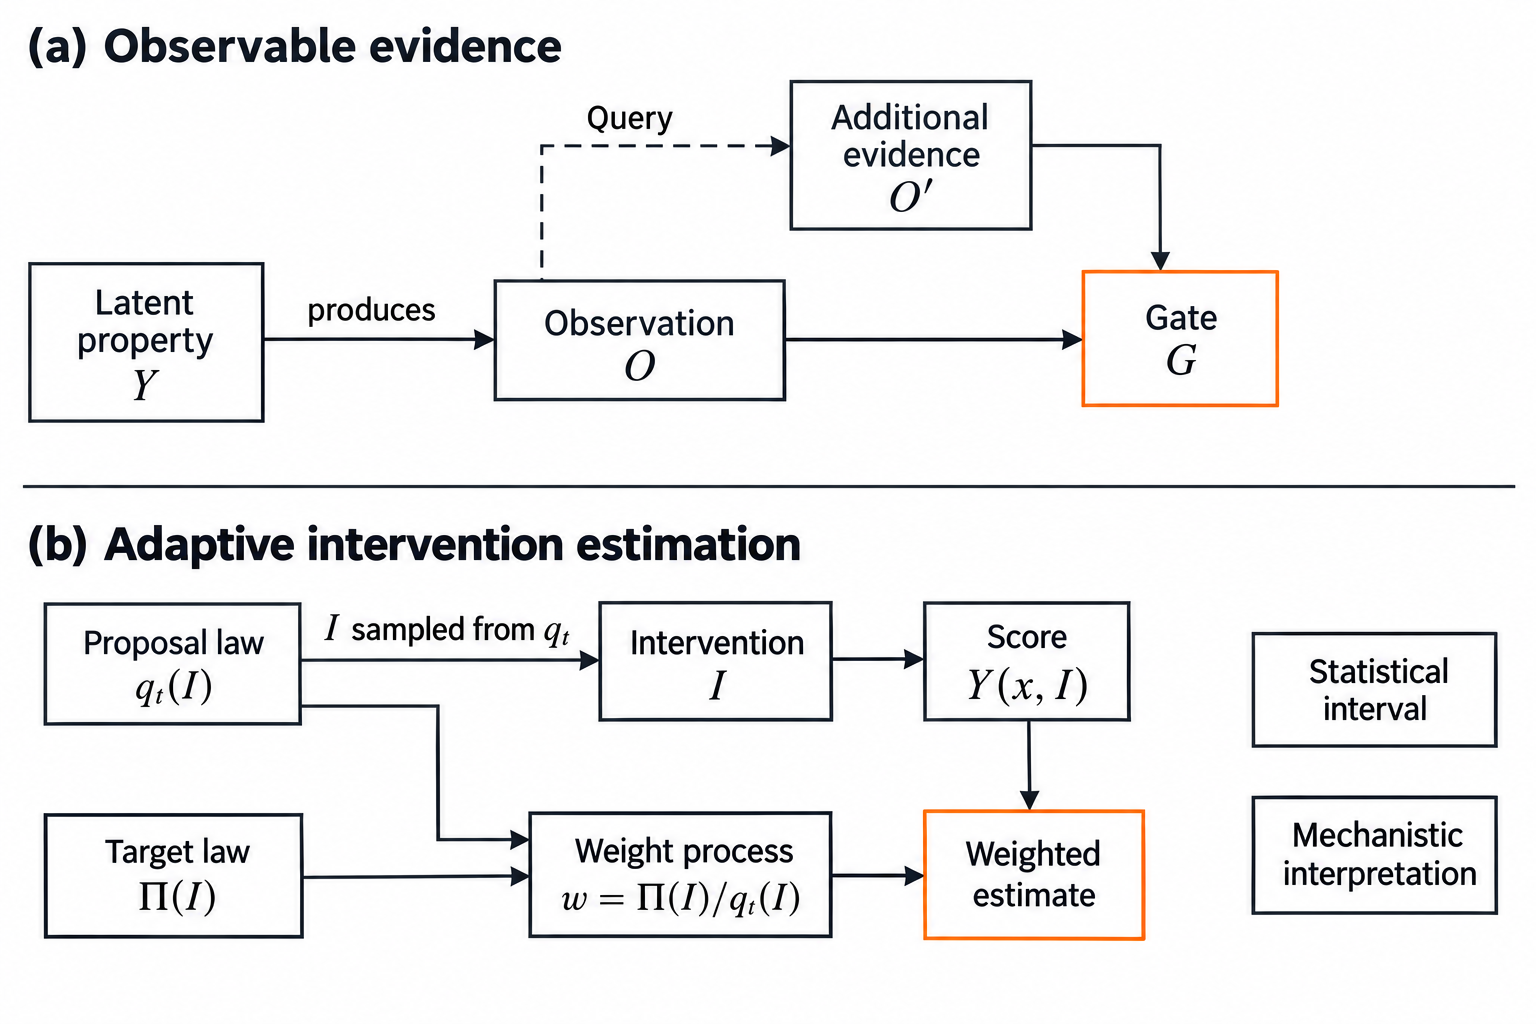
\includegraphics[width=\linewidth]{book/figures/assets/F25review.png}
\caption{Verification depends on evidence and inference. The upper $Y$ is a specified latent property; the lower $Y(x,I)$ is a declared intervention score. Additional queries can change observability. Only $q_t$ samples $I$; both densities are evaluated at that sample to form $w=\Pi(I)/q_t(I)$. Target support and bounded predictable weights are assumptions. An interval for the resulting estimand does not establish mechanistic truth.}
\label{fig:C25:overview}
\end{figure}

\section{Sparse features and their evaluation}\label{sec:C25:sparse}
Sparse autoencoders approximate an activation vector using a small number of learned dictionary features. A common objective combines reconstruction error with a sparsity constraint or penalty. Let $x$ be a model activation, $f(x)$ sparse feature activations, and $D$ a decoder dictionary. The reconstruction term $\|x-Df(x)\|^2$ measures approximation in activation space. It does not directly measure whether feature labels are correct or whether all behaviorally important structure is represented.

Anthropic's 2023 monosemanticity report applies dictionary learning to a small transformer and analyzes feature interpretation, intervention, splitting, and limitations~\cite{bricken2023monosemanticity}. OpenAI's 2024 sparse-autoencoder work studies scalable training and evaluation of reconstruction, sparsity, and feature quality~\cite{gao2024sae}. These are primary research contributions with different scopes. Neither establishes that a sparse representation is a unique, complete ontology of the model's concepts.

Feature interpretation must examine more than maximally activating examples. A feature can look clean at its strongest activations while responding to unrelated contexts at lower levels. Sampling only impressive examples introduces selection bias. Evaluation should include activation ranges, random examples, counterexamples, and downstream interventions. Automatic feature descriptions generated by another model require independent checking; a fluent label can rationalize a mixed feature.

Reconstruction and causal faithfulness can diverge. A dictionary can reconstruct common activation patterns well while missing rare behavior that matters for security or authorization. Conversely, a feature intervention can change behavior by moving computation off the model's natural activation manifold. The resulting effect is evidence about that intervention, not necessarily evidence that the feature normally causes the behavior in the same way.

For agent inspection, the relevant question is whether a feature-level explanation improves a concrete decision or detects a failure under held-out conditions. Compare it with simpler probes, input-output monitors, and executable checks at matched access and cost. A feature-based monitor should be tested after model updates, context compaction, and tool changes because its calibration may depend on the original distribution. Internal access can provide useful evidence while remaining an additional system component with its own drift and false-alarm behavior.

\subsection{The 2026 monitorability boundary}\label{sec:C25:monitorability2026}
The preceding circuit and dictionary methods are methodological foundations, not descriptions of the entire October 2026 inspection frontier. Contemporary oversight also uses monitors of reasoning traces, actions and tool results. These observations are complementary to internal activations: a readable trace is neither a complete causal account nor a proof that an accepted action satisfies its specification.

The August implicit-influence study compares matched nudges delivered as incidental contextual details or as explicit instructions to use and conceal the nudge~\cite{duzan2026implicit}. Across its tested task formats and extended-thinking models, behavioral influence can persist while trace-based detection weakens substantially in the implicit condition. Consequently, a monitor validated mainly on explicit concealment instructions can face a different observation problem in ordinary biased decision making. Its GPT-5-based judge does not establish that the influence is undetectable in principle; for Claude 4.5 runs the observed channel is an API summary rather than raw thinking. These are material access limits, not evidence that all reasoning traces are uninformative.

OpenAI's April 2026 release supplies datasets and metric code, but explicitly describes its public evaluation scaffold as illustrative and mocked, omitting restricted environments~\cite{openai2026monitorrelease}. The inspected \path{gmean_minimal_criterion} routine computes an effect-normalized detection bound with eligibility conditions; \path{bootstrapped_gmean_metric} separates eligibility selection from estimation and resamples within instance--arm strata. Its reported quantity must not be relabeled ordinary classifier accuracy or a direct measurement of complete causal faithfulness. Report the eligible-instance fraction alongside the conditional metric; an undefined case is not evidence of zero monitor error. The source revision is \texttt{d14f181a0623}; it was inspected, not executed~\cite{openai2026monitorcode}.

The September Astra system card supplies an additional current boundary: it distinguishes CoT-only, action-only and full-context monitors and reports reduced CoT monitorability relative to earlier models on its evaluations~\cite{openai2026astramonitor}. These are provider-reported configured results. Full-context access contains evidence absent from a trace-only monitor, so a comparison must hold observation scope fixed before attributing a difference to the monitor model. The existence of a full-context deployment monitor does not establish the same visibility for an application consuming an ordinary API response or a summarized reasoning field.

A discriminating experiment crosses actor checkpoint, monitor checkpoint, observation scope, context transformation and adversarial awareness. Freeze complete trajectories for the monitor comparison; separately rerun actors when studying how awareness changes behavior. Compressing a trajectory after the fact measures evidence loss to the monitor, whereas letting the actor reason under compacted context changes both behavior and available evidence. Preserve that distinction when interpreting the interaction. Evaluate sensitivity to implicit influence, false alarms on benign reasoning, alert delay relative to effect commitment, and compute cost. A monitor that identifies an error after an irreversible effect provides diagnostic evidence but has not demonstrated preventive control. An internal signal should become a deployment gate only after its held-out calibration and intervention consequences have been tested at the actual action boundary.

\section{Quality gates as fallible classifiers}\label{sec:C25:gates}
Let $Y=1$ mean a candidate satisfies the required property and $G=1$ mean a gate accepts it. Define sensitivity $s=\Pr(G=1\mid Y=1)$, false acceptance $f=\Pr(G=1\mid Y=0)$, and prevalence $\pi=\Pr(Y=1)$. Then
\begin{equation}
 \Pr(Y=1\mid G=1)=
 \frac{s\pi}{s\pi+f(1-\pi)}.
\end{equation}
Here $Y,G\in\{0,1\}$, $s,f\in[0,1]$, and $\pi\in(0,1)$ so both class-conditional gate rates are defined; acceptance also requires $s\pi+f(1-\pi)>0$. Degenerate single-class populations need their own conditional interpretation. The identity follows from Bayes' rule. It shows why an apparently accurate gate can produce unreliable accepted outputs when valid candidates are rare. It also shows why calibration measured on one candidate population cannot be transferred uncritically to another.

Repeated search changes that population. If an optimizer generates many candidates and retains one that passes, it increases exposure to the gate's blind spots. Under an illustrative independent-invalid-candidate model, the probability of at least one false acceptance among $n$ candidates is $1-(1-f)^n$. Independence rarely holds exactly, but the expression identifies the selection pressure. A gate evaluated only on ordinary samples can fail after adaptive optimization.

Adding another gate does not automatically multiply reliability. If gates share a model, prompt assumptions, or evidence source, their errors can be correlated. The joint false-acceptance rate is
\begin{equation}
 f_{12}=\Pr(G_1=1,G_2=1\mid Y=0).
\end{equation}
It equals the product of the two class-conditional marginal rates only when conditional independence is justified. Diversity of implementation and observation can reduce shared failure modes, but that effect requires measurement.

An unresolved verdict is operationally useful. It allows the system to distinguish lack of evidence from detected failure. However, unresolved cases must remain in reporting denominators. A gate can achieve high precision by accepting almost nothing; whether that is useful depends on coverage and task consequences. Report accepted precision, valid-candidate recall, unresolved rate, cost, and residual failure severity together.

Gate evaluation should include adversarially selected candidates and naturally occurring failures. Seeded faults establish sensitivity to known defect classes; natural audits reveal unanticipated classes. Neither alone estimates deployment risk. The candidate generator, gate, and final adjudicator should have separate evaluation splits where possible. Otherwise the same held-out examples can leak into both optimization and assessment, creating an appearance of independent verification without actual independence.


\section{Dynamic tests and requirement-grounded witnesses}\label{sec:C25:testjack}
TestJack audits benchmark-passing coding trials by generating tests tied to prompt requirements, checking them against a reference solution, and reviewing whether failures represent genuine requirement violations~\cite{yao2026testjack}. Its distinction between insufficient tests and underspecified prompts is essential: disagreement with the reference is not enough to refute a candidate. The paper reports substantial refutations in its audited passing-trial corpus; that proportion is not a prevalence estimate for all coding-agent executions.

The method's witness structure has three obligations. The test must correspond to a required behavior, pass on the reference, and fail on the candidate. The executable conditions are reproducible, but the requirement correspondence remains interpretive. A faulty reference or ambiguous prompt can invalidate the inference. A reviewer agent reduces some mistakes but does not become an oracle merely because its role is called reviewer.

A stronger causal ablation keeps the candidate set and execution environment fixed while varying requirement grounding, reference validation, and review. Measure how many proposed witnesses survive independent adjudication and what defect classes they expose. Also examine false refutations: a method that discovers many failures by imposing extra requirements can reduce a leaderboard score while making the evaluation less valid.

Witness sharing across trials can amortize cost. If several candidates fail the same requirement, one validated test can inspect them all. This changes the unit of evidence: outcomes share a task and a discovered witness, so they are statistically dependent. Uncertainty should reflect that clustering. Randomly auditing trials can estimate properties of the declared audit population, but adaptive witness reuse and selective follow-up require a carefully described sampling scheme.

The implementation path should preserve the original repository, candidate patch, reference patch, generated witness, native test runner, and adjudication record. An artifact link or algorithm description does not establish that all pieces are available at an immutable revision. Until the exact implementation is inspected and run, report the method and author results separately from reproduction. This is particularly important for evaluator evolution, where changing a prompt or test-generation model can alter the measured defect population.


\section{Judging long multimodal trajectories}\label{sec:C25:judges}
Long computer-use trajectories challenge evaluators through observation volume, hidden state, and instruction-specific constraints. A judge may accept a visually convincing outcome while missing a wrong recipient, incorrect folder, or unrequested side effect. Conversely, it may reject a valid trajectory because the decisive evidence lies in an intermediate application state rather than the final image.

AgentHorizon uses paired instruction-trajectory relationships to probe these distinctions~\cite{corpus261011050}. Its design motivates evaluating false acceptance and false rejection separately rather than relying on a single agreement rate. A judge that accepts almost every plausible workflow can appear competent on a positive-heavy dataset. Balanced metrics help, but they do not replace a clear definition of the underlying positive and negative populations.

Evidence access should be controlled experimentally. Compare final-state observation, full trajectory, searchable artifact logs, and authoritative application queries. These conditions test different capabilities. Giving one judge an interactive tool harness and another only a fixed image sequence confounds model quality with evidence access. Tool-enabled judging also incurs latency and cost, and tools can fail or expose misleading state.

A useful implementation separates evidence retrieval from verdict generation. The judge identifies required predicates, retrieves supporting observations, and links each verdict to the corresponding evidence. This improves auditability but does not guarantee correctness. Evaluate whether cited observations actually establish the predicate and whether omitted constraints were checked. A verbose explanation can otherwise hide a shallow verdict behind extensive irrelevant evidence.

Trajectory compression is another treatment. Summaries can reduce evaluator cost while deleting the rare event that distinguishes success from failure. Compare compression methods on matched task families and include perturbations that move decisive evidence earlier or later in the history. Report the cost of reconstructing original observations. If the judge needs raw evidence after every difficult case, the summary's apparent savings may not survive end-to-end accounting.


\section{Verification experiments and implementation traceability}\label{sec:C25:experiments}
A verification study should predeclare the property, candidate population, observation interface, and adjudication process. It should also distinguish discovery from confirmation. Cases used to design a new gate belong to development; untouched cases test whether the gate generalizes. Repeatedly inspecting failures and adjusting the gate against the same holdout turns the holdout into a training resource even if no model weights change.

The implementation ledger links a source claim to an equation or algorithm, a versioned code path, configuration, dataset split, and observed result. For ROME, inspect the intervention and editing implementation separately; a successful edit does not validate every localization claim. For sparse autoencoders, inspect training, feature extraction, and downstream metrics separately. For executable witnesses, preserve the native test environment and the requirement argument. These boundaries prevent one successful component from lending unwarranted credibility to another.

Negative controls are particularly valuable. Patch a random activation site, use an irrelevant feature description, supply a test that distinguishes an incidental reference choice, or give a judge a trajectory for a related but incompatible instruction. A valid verification method should reject or limit these controls appropriately. Failing a negative control identifies a concrete weakness in causal interpretation or specification handling.

Uncertainty must follow the sampling unit. Multiple prompts for one fact, several features from one model layer, and many candidate patches for one task are not independent replications of the entire method. Use task-, fact-, model-, or repository-level grouping as appropriate. Report heterogeneity rather than only an aggregate mean, especially when rare errors have disproportionate consequences.

The practical implication is that verification is an evidence-producing system with its own model, tools, data, and failure modes. It should be versioned, monitored, and independently evaluated. Internal inspection can reveal useful mechanisms; executable checks can falsify artifacts; structured evidence can expose unsupported claims. Their combined strength comes from complementary observation and intervention, not from relabeling a second model as an infallible critic.

\section{A worked gate analysis with adaptive selection}\label{sec:C25:workedgate}
Consider a system that proposes a code change, obtains a test verdict, asks a model critic for approval, and publishes the accepted artifact for review. There are at least four distinct latent events: the patch satisfies the requirement, the test suite covers the relevant behavior, the critic interprets the evidence correctly, and the published artifact is the one that was checked. A failure at any stage can produce a misleading acceptance. Calling the arrangement a verification pipeline does not remove those events from the analysis.

Begin with the artifact-binding obligation. The test runner records digest $d_1$, while the publication tool is about to send digest $d_2$. If $d_1\ne d_2$, the gate should reject or rerun regardless of the critic's confidence. This is a deterministic check over recorded identities. If the digests match, the system has established that evidence and artifact correspond, but it has not established that the tests cover the specification. The distinction allows an engineering invariant to be enforced without claiming an unavailable semantic oracle.

Next consider a candidate that passes all visible tests by special-casing the tested examples. A model critic may notice the shortcut, but it may also infer that the behavior is acceptable because the benchmark passes. A requirement-grounded witness can target an untested input implied by the prompt. If the witness fails on the candidate and passes on the reference, the remaining question is whether its expectation actually follows from the task. An independent reviewer should be shown that question without being encouraged to treat the reference's incidental choices as requirements.

Now add adaptive search. The agent sees a rejection and revises the patch. The resulting candidates are not independent draws from a fixed distribution: each can be optimized against prior feedback. A false-acceptance rate measured before this interaction may no longer apply. To obtain a union bound over $n$ attempts, one sufficient condition is a bound $f_t$ on the conditional probability of false acceptance at attempt $t$ given the entire previous search history. Then the probability of any false acceptance is at most $\min(1,\sum_t f_t)$. Marginal calibration on unrelated samples does not establish these conditional bounds.

The implementation consequence is to retain the search history and gate version. If a candidate generator is allowed to query the gate repeatedly, the evaluation must expose that access and include it in the budget. A final accepted artifact should identify how many candidates were considered and whether the gate's feedback was visible during revision. Otherwise two systems with the same final test suite can have different effective opportunities to exploit it.

A holdout gate can reduce direct adaptation, but it introduces its own governance problem. If researchers repeatedly inspect holdout failures to improve the system, the holdout gradually becomes development data. Rotating tasks or using a genuinely untouched confirmation set can help, provided the task distribution remains relevant. A smaller untouched sample may yield wider uncertainty than a large heavily reused benchmark. Scientific reporting should preserve that uncertainty rather than prefer the larger but compromised number.

Threshold selection also depends on consequence. A gate used to prioritize human review has a different loss function from a gate that authorizes external publication. Let $c_{FA}>0$ be the cost of false acceptance and $c_{FR}>0$ the cost of false rejection. For $q=\Pr(Y=1\mid O)$ conditional on the information $O$ actually available to that decision, accepting has expected error cost $c_{FA}(1-q)$ and rejecting has expected error cost $c_{FR}q$ under a simplified two-action model. Acceptance is favored when $q\geq c_{FA}/(c_{FA}+c_{FR})$, with either decision permissible at equality. An estimated score requires validation in the corresponding decision population; marginal calibration on unrelated candidates does not supply this posterior when additional covariates change the costs or error distribution. The formula does not make either probability or cost available automatically.

An unresolved or review action changes that decision problem. Review can acquire additional evidence at cost, and the reviewer is also fallible. A rational policy compares expected residual loss after review with immediate acceptance or rejection. In practice these quantities are difficult to estimate, so applications often use hard rules for consequential effects and probabilistic gates for lower-impact filtering. The rules should be justified by the action boundary, not by an arbitrary global confidence threshold.

This analysis transfers to internal model monitors. Suppose a sparse feature is associated with a concerning behavior and triggers a warning. The feature's activation can be a useful signal without being a complete causal explanation. Calibration depends on model revision, context distribution, and intervention history. If the deployment policy changes behavior in response to the monitor, the observed data distribution changes too. A monitor evaluated only before intervention can therefore become miscalibrated after it is embedded in a control loop.

The discriminating experiment has separate discovery, calibration, adaptive-attack, and confirmation phases. Discovery identifies candidate signals or tests. Calibration estimates their behavior on a declared population. Adaptive evaluation allows a bounded optimizer to search for accepted failures. Confirmation evaluates the final fixed configuration on untouched cases. Report how candidates, tasks, and model families overlap between phases. This makes the independence claim inspectable rather than relying on the label held out.

Finally, preserve the distinction between a falsifying witness and a comprehensive safety claim. One replayable counterexample can refute a universal assertion about a gate. The absence of a counterexample in a finite search cannot establish that no accepted failure exists. It can support a bounded empirical statement about the search procedure, budget, and task population. That statement is valuable when accurately scoped. Inflating it into certification makes the evidence less useful precisely because it hides the operating conditions under which the gate was actually examined.

The ROME implementation makes this separation concrete. Its published causal-tracing experiment exposes a patching routine and hidden-flow calculation, while the model-editing module exposes the function that applies ROME updates\cite{meng2022rome}. These are distinct execution paths with distinct claims: restoring selected activations tests mediation under an intervention; applying an update tests whether a weight change produces the desired association and preserves specified neighboring behavior. A reproduction ledger should not mark both claims reproduced because only the editing demo ran. The sparse-autoencoder implementation likewise separates encoding and decoding in its Autoencoder class\cite{gao2024sae}. Reconstructing activations through those functions establishes numerical behavior of the learned dictionary, while interpreting a feature and evaluating its downstream causal effect requires additional experiments. Record the model checkpoint, selected layer, activation normalization, feature selection rule, intervention magnitude and metric. These fields identify where two apparently contradictory analyses may actually differ. Code availability therefore strengthens inspectability without collapsing the distinction between a reachable function, an executed experiment and a supported scientific conclusion.

In particular, the inspected ROME source contains \path{trace_with_patch}, \path{calculate_hidden_flow}, \path{apply_rome_to_model} and \path{execute_rome}. Their presence was checked; no execution result is asserted here. Pinning these callables to a revision and running the associated controls is the implementation step required before an independent reproduction claim.

